\section{Zwischenwertsatz}
Sei $f: [a,b] \to \R$ eine stetige reele Funktion, die auf einem Intervall
definiert ist mit o.B.d.A $f(a) \leq f(b)$. Dann gilt:\\
{\small $\forall u \in [f(a), f(b)] \; \exists c \in [a, b]$ so dass $f(c) = u$} \\
\vspace{-0.2cm}
\hspace{5.cm}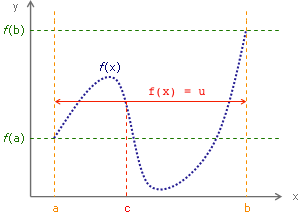
\includegraphics[scale=0.4]{zwischenwertsatz.png}

\vspace{-1cm}
\subsection{Beispiel (Fixpunkt)}
Sei $f: [0,1] \to [0,1]$. Zeige: $f$ hat einen Fixpunkt, d.h. es gibt ein $x
\in [0,1]$ derart, dass $f(x) = x$.

Man erzeugt die Funktion $g: [0,1] \to \R, g(x) := f(x) - x$. Es gilt: $f(x) =
x \Leftrightarrow g(x) = 0$, d.h. ein Punkt x ist genau dann ein Fixpunkt von
$f$ wenn er eine Nullstelle von $g$ ist. Es ist zu zeigen, dass $g$ immer eine
Nullstelle auf $[0,1]$ hat. Als Differenz von zwei stetigen Funktionen ist $g$
stetig. Weil ausserdem $f(x) \in [0,1] \; \forall x \in [0,1]$ gilt, ist $g(0)
\geq 0 \geq g(1)$. Da $g$ stetig ist, gibt es daher nach dem Zwischenwertsatz
ein $x \in [0,1]$ mit $g(x) = 0$ und somit gibt es $f(x) = x$.
